\begin{frame}
	\begin{center}
		\Huge Grafikdesign
	\end{center}
\end{frame}

\begin{frame}{Grafikdesign}
    \begin{figure}
        \includegraphics[width = 10cm]{bilder/Foyer_Zeittafel.png}
        \caption{Erstellung des Foyer}
    \end{figure}
\end{frame}

\begin{frame}{Grafikdesign}
    \begin{figure}
        \includegraphics[width = 10cm]{bilder/Hausmeisterraum_Zeittafel.png}
        \caption{Erstellung des Hausmeisterraumes}
    \end{figure}
\end{frame}

\begin{frame}{Grafikdesign}
    \begin{figure}
        \includegraphics[width = 10cm]{bilder/Hausmeisterraum_Details.png}
        \caption{Details im Hausmeisterraum}
    \end{figure}
\end{frame}




\begin{frame}{Grafikdesign}
	\begin{minipage}[v]{0.32 \textwidth}
		\begin{figure}
			\includegraphics[width=\textwidth]{bilder/Bioraum.png}
			\caption[Bioraum]{\newline Der Bioraum}
			\label{fig:Bioraum}
		\end{figure}
	\end{minipage}
\hfill
\begin{minipage}[v]{0.32 \textwidth}
	\begin{figure}
		\includegraphics[width=\textwidth]{bilder/Info-Raum.png}
		\caption[Inforaum]{\newline Der Inforaum}
		\label{fig:Inforaum}
	\end{figure}
\end{minipage}
\hfill
\begin{minipage}[v]{0.32 \textwidth}
	\begin{figure}
		\includegraphics[width=\textwidth]{bilder/Physikraum.png}
		\caption[Physikraum]{\newline Der Physikraum}
		\label{fig:Physikraum}
	\end{figure}
\end{minipage}

\end{frame}

\begin{frame}
    \begin{figure}
    	\begin{minipage}{0.32\textwidth}
    		\begin{figure}
    			\includegraphics[width=\textwidth]{bilder/kt_farbverlauf}
    			\label{fig:kt_farbverlauf}
    		\end{figure}
    	\end{minipage}
        \hfill
        \begin{minipage}[v]{0.32\textwidth}
            \begin{figure}
                \includegraphics[width=\textwidth]{bilder/kt_schule.png}
                \label{fig:kt_schule}
            \end{figure}
        \end{minipage}
        \hfill
        \begin{minipage}[v]{0.3\textwidth}
            \begin{figure}
                \includegraphics[width=\textwidth]{bilder/kt_tetris.png}
                \label{fig:kt_tetris}
            \end{figure}
        \end{minipage}
        \caption{drei unterschiedliche kleine Treppenhäuser}
    \end{figure}
\end{frame}

\begin{frame}
	\frametitle{Gang- und Raumszenen}
	\begin{itemize}
		\item für jede Szene gibt es eine eigene Klasse
		\item Szenenwechsel per Pfeil in den Gängen
		\item Eintritt in Räume über die Türen
		\item in jeder Szene taucht der Spieler auf
	\end{itemize}
\end{frame}

\begin{frame}
	\begin{figure}
		\includegraphics[width = 11 cm]{bilder/Chemiegang.png}
		\caption{Chemiegang}
	\end{figure}
\end{frame}

\begin{frame}
	\frametitle{Aufbau der Szenenklassen}
	\begin{figure}
		\includegraphics[width = 11 cm]{bilder/CodeSzene.png}
		\caption{Beispielcode (Chemiegang)}
	\end{figure}
\end{frame}

\begin{frame}
	\frametitle{Das Pfeilobjekt}
	\begin{minipage}{0.45\textwidth}
		\begin{itemize}
			\item formale Parameter:
			\begin{itemize}
				\item Originalszene
				\item Zielszene
				\item Richtung
			\end{itemize}
			\item getSprite(int Richtung)
			\item Festlegen der Position des Pfeils abhängig von der angegebenen Richtung
		\end{itemize}
	\end{minipage}
	\begin{minipage}{0.45\textwidth}
		\begin{figure}
			\includegraphics[width = 5 cm]{bilder/Pfeile.png}
			\caption{Pfeile}
		\end{figure}
	\end{minipage}
\end{frame}

\begin{frame}
	\frametitle{Das Pfeilobjekt}
	\textbf{Updatefunktion}
	\begin{itemize}
		\item Wenn das Objekt angeklickt wird:
		\begin{itemize}
			\item Austausch der alten gegen die neue Szene im Szenenstapel
			\item Timer für das Inventar
		\end{itemize}
	\end{itemize}
\end{frame}

\begin{frame}
	\frametitle{Das Türobjekt}
	\begin{minipage}{0.65\textwidth}
		\begin{itemize}
			\item formale Parameter:
			\begin{itemize}
				\item x-Koordinate
				\item y-Koordinate
				\item Originalszene
				\item Zielszene
			\end{itemize}
			\item unsichtbares Objekt
			\item Updatefunktion
			\begin{itemize}
				\item Austausch der Szenen im Szenenstapel
			\end{itemize}
		\end{itemize}
	\end{minipage}
	\begin{minipage}{0.3\textwidth}
		\begin{figure}
			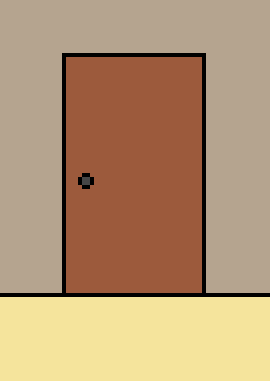
\includegraphics[width = 3.5 cm]{bilder/Tür.png}
			\caption{Tür}
		\end{figure}
	\end{minipage}
\end{frame}

\begin{frame}
	\frametitle{Position des Spielers}
	\begin{minipage}{0.6\textwidth}
		\begin{itemize}
			\item Methode getRandomX()
			\begin{itemize}
				\item Festlegen einer zufälligen x-Koordinate für die Spielfigur
			\end{itemize}
		\end{itemize}
	\end{minipage}
	\begin{minipage}{0.35\textwidth}
		\begin{figure}
			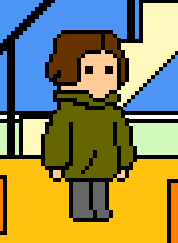
\includegraphics[width = 3.75 cm]{bilder/Spieler.png}
			\caption{Spielfigur}
		\end{figure}
	\end{minipage}
\end{frame}

\begin{frame}
	\begin{figure}
		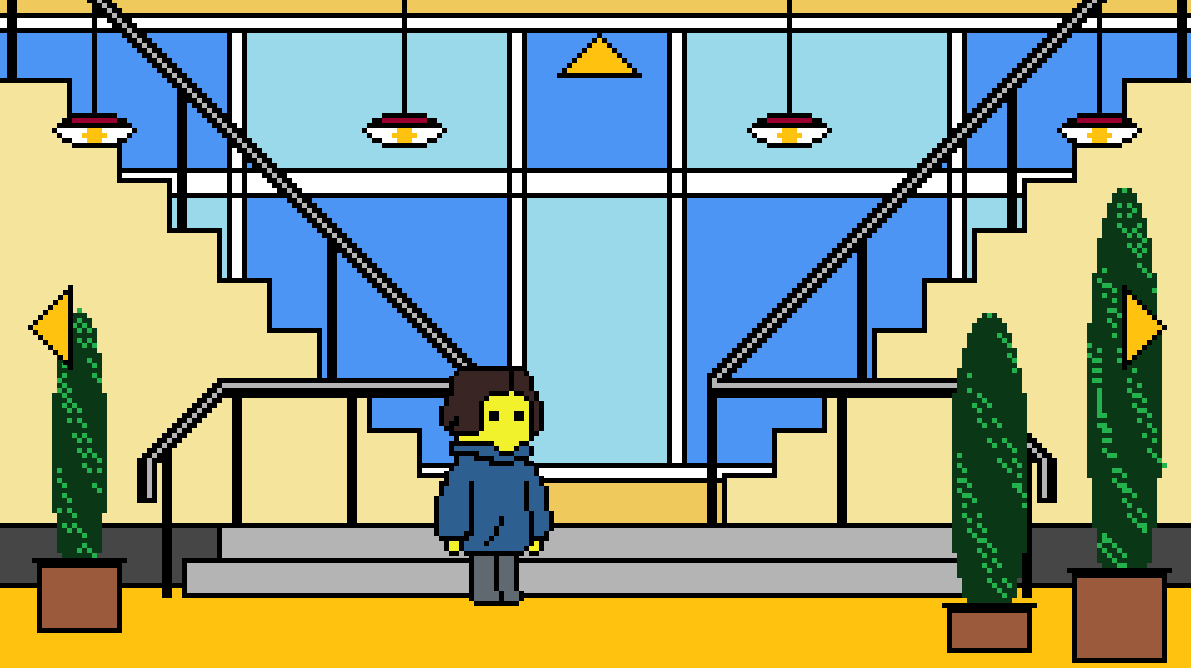
\includegraphics[width = 11 cm]{bilder/Foyer.png}
		\caption{Foyer}
	\end{figure}
\end{frame}
